\documentclass [french,12pt]{article}
\usepackage[french]{babel}
\usepackage[utf8]{inputenc} 
\usepackage{graphicx}
\usepackage{enumerate}
\usepackage{amsmath,amsfonts}


\title{Rapport de la première soutenance}

\author{\includegraphics[scale=0.4]{team} \andcr Becquet Antoine (becque\_a) \andcr Cavillon Louise (cavill\_l) \andcr Lahalle Arnaud (lahall\_a) \andcr Helouis Guillaume (heloui\_g)}
\date{22 Octobre 2012}
\begin{document}
\clearpage
\tableofcontents
\clearpage



\section{Introduction}

Oyez chers lecteurs ! Vous voici maintenant en contact avec le rapport de première soutenance du groupe" Renaissance du travail totalitaire" ! 
Notre mission en tant que étudiants en seconde année de l'EPITA  : réaliser un logiciel de reconnaissance de caractère, communément appelé OCR.
Nous allons dans un premier temps vous présenter notre équipe, puis la distribution des tâches à réaliser pour mener notre projet à bien et enfin exposer ce qui a été fait . Bonne lecture !  


\subsection{Un OCR ? késako?}

Le logiciel que nous devons réaliser reconnait les caractères manuscrits et imprimés. Plus précisément, le logiciel a la capacité d' "apprendre" à reconnaître des écritures ou symboles particuliers. En effet,  si un utilisateur lui fournit des documents contenant son écriture en format normalisé, celui-ci parviendra à créer un profil relié directement à ce type d'écriture très particulier.
Ensuite, par une simple procédure, l'utilisateur sera capable de passer d'une image contenant du texte à un texte utilisable et donc, transformable.

\subsection{L'équipe ! }
\subsubsection{Antoine "Reynova" Becquet : the Big Boss qui a le fouet}


\subsubsection{Louise "Amaterasu" Cavillon}
C'est avec une certaine appréhension couplée avec un curiosité intense que j'ai pris connaissance de ce sujet ! En effet, parvenir à comprendre les algorithmes mis en jeu pour passer d'un support de type image à un texte directement utilisable et modifiable est très intéressant ! Cependant, leurs complexités et difficultés sont impressionnantes pour un débutant en traitement d'image. En ce qui concerne le groupe, le sérieux que je recherche est au rendez-vous et l'entraide présente ! Il est donc agréable de travailler et de nous perfectionner dans le merveilleux monde de l'OCR ! 

\subsubsection{Guillaume "Guigui" Helouis}

Le projet de cette année va certainement m'en apprendre beaucoup. 
L'environnement Unix est vraiment très intéressant et riche en possibilités.
\\
Utilisation de VIM, fonctionnement des Makefile... Des outils qui demandent un temps d'adaptation, mais qui se révèlent extrêmement puissants.
Pour notre OCR, j'ai réfléchi à l'implémentation de divers algorithmes permettant de séparer l'image originale en blocs de textes distincts.


\subsubsection{Arnaud "Nono" Lahalle}
Etudiant en informatique en deuxième année à Epita (Ecole pour l'informatique et les technologies avancées).
Ce projet a l'avantage d'être un projet assez simple à comprendre tout en étant assez complexe à mettre en oeuvre.  
Mon but dans le projet consiste à faire tourner l'image afin que la détection de caractère soit plus précise et que le résultat soit de meilleurs qualité.


\section{Organisation}
\begin{itemize}
\item{Pré-traitement de l'image; Détection de l'angle de rotation et rotation : Arnaud,  Louise}
\item{Détection des lignes : Antoine}
\item{Détection des zones de texte : Guillaume}
\item{Site web : Louise}
\end{itemize}

\section{Le pré-traitement de l'image}

Lorsque l'utilisateur va donner une image au logiciel, elle peut ne pas être "parfaite". En effet, les lignes peuvent ne pas être horizontales, il peut y avoir une couleur de fond autre que blanc ou encore avoir du "bruit", c'est à dire des pixels dont la couleur tranche avec celles des pixels voisins et qui parasitent l'image. Différents traitement sont donc nécessaires pour corriger ces imperfections.
Nous allons maintenant vous présenter les transformations et algorithmes que nous avons retenu.

\subsection{La rotation}

Dans le cas où les caractères sont tordus  (à cause d'une rotation d'un certain angle intrinsèque au document), leurs traitement sera accompagné d'erreurs. Par pallier à cela, il nous faut donc d'abord détecter un angle de rotation qui facilitera l'identification des caractères puis l'appliquer.

\subsection{Détection de l'angle}

\begin{center} 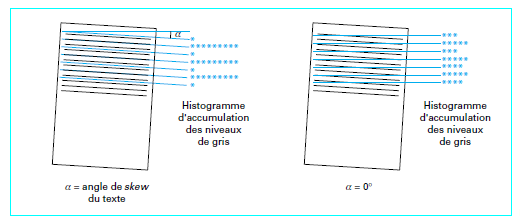
\includegraphics[scale=1.00]{rotation_arnaud} \end{center}
\\

Nous allons vous décrire l'algorithme que nous avons utilisé dans ce but.
Il s'agit de l'algorithme de Postl qui s'applique à des images à niveaux de gris ou biniveau. La méthode opère à partir d'un sous-échantillonnage de 1/N en hauteur et de 1/P en largeur et consiste à :
\\
\begin{itemize}
\item Tracer virtuellement sur l'image N lignes parallèles et équidistantes faisant un angle de alpha avec l'horizontale ;
\\


\item Calculer le long de chacune de ces N lignes la somme P des niveaux de gris rencontrés en prenant 1 pixel sur P seulement ;
\\
\item Calculer sur l’ensemble des N lignes la somme P des carrés des différences des sommes l d’une ligne i à la suivante i+1 ;
\\
\\
\\
$\sum_{i=1}^{n} (S_{ligne i}-S_{ligne i+1})^{2}$
\\
\\
\\
\item Faire varier l’angle alpha, et trouver la valeur pour laquelle cette valeur P passe par un maximum.

\\

\end{itemize}
\\
Cela revient à cumuler les projections de pixels le long d’une ligne inclinée
\\ et à chercher l’angle pour lequel ces accumulations
 \\se mélangent le moins quand on passe d’une ligne à la suivante.
\\
Nous mettrons ainsi la valeur de P et de l'angle dans un tableau, puis nous le trierons afin de récupérer la valeur de l'angle alpha pour lequel P soit la plus grande valeur de la liste.
\\
Mais cet algorithme n'est pas encore au point, il s'agira donc d'un point à améliorer pour la soutenance finale.

\subsection{Application de l'angle de rotation adéquate}

Pour la première soutenance l'algorithme de rotation sera assez simple. Il consistera à parcourir toutes l'image que l'on veut tourner. Puis pour chaque pixel nous calculerons sont image avec une rotation d'angle alpha en fonction du point de rotation. (Les coordonnées du point de rotation correspondra au centre de l'image).
Pour effectuer cette rotation nous utiliserons les formules de trigonométrie. Il ne faut non plus oublier que l'axe des ordonnées est inversée quand on parcourt une image. 
Soit (x1,y1) les coordonnées de (x,y) après la rotation d'angle alpha et (cx,cy) le milieu de l'image (Le centre de rotation)

\[x1 = (x-cx) * \cos \alpha + (y-cy) * \sin \alpha + cx \]
\\
\[y1 = (y-cy) * \cos \alpha + (cx-x) * \sin \alpha + cy \]

Or cette méthode présente un défaut majeur quand on effectue les calculs ont obtient les coordonnées du nouveau pixel en floatant. Ainsi on est obligé de troncaturer ces valeurs pour les placer dans l'image. Donc sur certains pixels de la nouvelle image il y aura donc des "artefacts", certains trous (des pixels blancs) seront présents entre les pixels noirs. Il s'agira donc d'un point à améliorer pour la seconde et dernière soutenance. 

La seconde méthode est appelée rotation par bilinéarisation. Au lieu de parcourir tout les pixels de l'image de départ, nous allons calculer la rotation inverse des pixels de l'image d'arrivée. Pour obtenir les données des pixels de l'image d'arrivée.  
\\
\subsection{Effacement du bruit}

Comme dit précédemment, le but de ce traitement est d'atténuer les imperfections de l'image donnée.
Pour ce faire, nous faisons un parcours de cette image. Au niveau du pixel courant, nous regardons la couleur des huit pixels qui l'entoure et en faisons une moyenne. Cette couleur résultant de la moyenne va alors remplacer l'ancienne couleur du pixel courant. Lors des cas particuliers comme les bords ou les coins de l'image, où il n'y a pas huit pixels autour du pixel courant.
Voici un schéma explicatif de la détection : 

\begin{center} 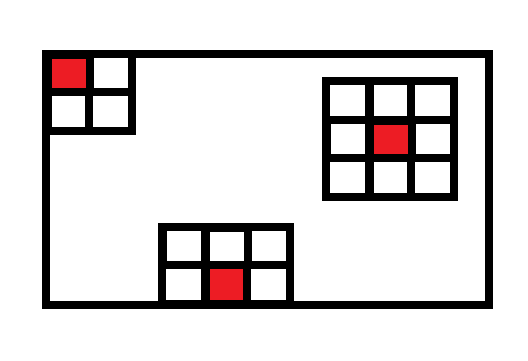
\includegraphics[scale=0.4]{a} \end{center}
\\
Sur cette image, le pixel rouge est le pixel courant  et les autres pixels en blancs sont ceux dont on récupère l'image. Les différents cas sont traités : pixel quelconque entouré de huit autres pixels, pixel particulier d'un coin et pixel d'un bord de l'image.


\subsection{Binarisation}

Notre algorithme de binarisation est simple mais très rapide !  Nous parcourons l'image et lorsque nous sommes sur le pixel courant, on récupère sa couleur. \\
Si elle est supérieure ou égale à la moyenne entre la couleur blanche et noire, on met le pixel courant à blanc, sinon, à noir.\\


\subsection{Amplifier les marques des caractères}

Dans le cas où l'image que l'utilisateur donne, a un fond d'une couleur différente de blanc, il faut que notre logiciel soit en mesure de distinguer fond (dont la couleur doit changer) et les objets que sont les caractères. 
Pour atteindre cet objectif, il faut effectuer une sorte de seuillage. \\
Nous parcourons donc l'image et récupérons son niveau de gris. La valeur obtenue (qui est un entier) appelée n, entraînera l'incrémentation du compteur nb (initialisé à zéro au départ dans toutes les cases) dans la case n. \\
Cela va nous permettre de recréer virtuellement un histogramme : graphique en deux dimensions montrant à l'aide de "pics" le nombre de pixels qui ont un niveau de gris en commun. Sur cet objet, les niveaux de gris sont classés par ordre croissant.  A un niveau de gris particulier, on va pouvoir noter une très grande différence du nombre de pixels ayant une valeur de gris i et un niveau de gris i+1. Ce passage est défini comme le seuil. C'est lui qui nous donnera une indication de la valeur de niveau de gris et par conséquent, nous permettra de ne prendre en compte que les caractères ou le fond.\\

\begin{center} 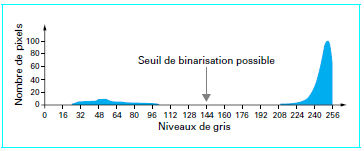
\includegraphics[scale=1.50]{seuil} \end{center}

\newpage

\section{Détections}
\subsection{Détections des lignes}
\subsection{Détections des zones de texte}

\section{Le site web}
Pour que des personnes extérieures au projet puissent suivre notre avancée, nous avons développé un site web avec le logiciel wordpress. Il est disponible à http://www.opticalcharacterrecognition.wordpress.com/ . Sont disponibles des présentations de l'équipe "Renaissance du travail totalitaire", le téléchargement de ce présent rapport et le logiciel d'OCR. Nous avons choisi un thème très simple mais toutefois en lien direct avec les caractères -thème principal de l'OCR - : Pilcrow. Celui-ci nous permet de mettre une image de fond et une image d'en-tête personnalisées. Nous avons respectivement choisi l'image d'un parchemin et l'image d'un chameau en calligramme car ils rappellent tout deux l'essence même du projet : l'écriture sous toute ses formes ! De plus, le chameau nous semblait tout à fait adapté aux conditions de réalisation du projet ! 


\section{En conclusion}
\end{document}
